\chapter{微分方程}
\section{分离变量}
首先什么是微分方程呢?如果我们不知道一个函数$y(x)$的表达式,但是知道$\frac{\opd y}{\opd x}$与$x$、$y$的一些关系,然后就能把$y(x)$的表达式求出来,这样的方程就叫作微分方程。

举个栗子,一个地方的人口越多,人口增长得就越快。我们建立一个简单的模型,设人口为$y$,时间为$t$,那么$\frac{\opd y}{\opd t}=a y$,$a$是一个比例系数。可以这样解这个方程:
\begin{align*}
\frac{\opd y}{\opd t}&=a y \\
\frac{\opd y}{y}&=a \opd t
\internote{(现在$y$在方程的一边,$t$在方程的另一边,这种方法叫做\emph{分离变量})}
\ln y&=a t+C
\internote{(两边同时积分,本来都有积分常量,但是只要写一个$C$,另一个可以移到对面)}
y&=\exp(a t+C) \\
&=y_0 \exp a t
\end{align*}

其中$y_0=\exp C$,表示初始时的人口。如果初始时一个人都没有,以后当然不会有人出现。这就是高中生物课本上的J形增长曲线,所以生物学中很多图的纵坐标是数量的对数。

【练习】S形增长曲线满足$\frac{\opd y}{\opd t}=a y(K-y)$,先猜一猜这个方程是什么意思,然后把它解出来。

只有$\frac{\opd y}{\opd t}=a y$ 是无法确定$y_0$ 的,需要一个另外的条件才能确定,比如直接告诉你初始人口,也可以是一年后的人口。但是只要有一个条件,其他时候的人口就确定了,如果有更多的条件,就有可能自相矛盾(比如某些高中物理老师拍脑袋想出来的电磁感应题)。这种条件叫做\emph{边界条件}。(有些地方把边界条件叫作初始条件,我自己也分不清楚)

积分常量没有确定的时候,微分方程的解叫做\emph{通解},而积分常量确定之后,微分方程的解叫做\emph{特解}。上面这个方程中有$y$的一阶导数,所以叫做一阶微分方程。$n$阶微分方程需要$n$次积分才能解出来,通解有$n$个积分常量,需要$n$个边界条件才能确定特解。

话说有单位的东西叫作“量”,没有单位的东西叫作“数”,这件事情等到量纲分析再仔细讲。

悲剧的是,很多微分方程都是解不出来的(用初等函数表示)。就算能分离变量,接下来的积分也不一定能积出来。能用分离变量法解出来的都是一些最简单的微分方程,但是一般够用了,复杂的方法比如积分因子和花式换元法以后再讲。($\leftarrow$有生之年)
\section{线性常系数齐次微分方程;直接猜出解}
把待求函数设为$y(x)$,现在来看另一种简单的微分方程:
\begin{equation*}
a_0 y+a_1 y'+a_2 y''+\dots+a_n y^{(n)}=0
\end{equation*}

线性在数学的不同领域中有不同的意思,在这里是指方程中$y$和它的各阶导数最多只有一次项,而没有相乘的项,比如$y^2,y'^2,y \cdot y'$都不行。常系数指的是$y$和它的各阶导数不会和$x$相乘,也就是说$a_0,a_1,a_2\dots$都是常量。齐次指的是方程右边为零。这些名字现在记不住也没关系,以后会知道为什么这样的方程特别简单。

现在可以猜:$y=\rme^{\rmi k x}$。这样$y'=\rmi k \rme^{\rmi k x}=\rmi k y$,$y^{(n)}=(\rmi k)^n y$,这就是指数函数的好处。

代入方程得到$a_0 y+a_1 \rmi k y+a_2 (\rmi k)^2 y+\dots+a_n (\rmi k)^n y=0$,约掉$y$得到$a_0+a_1 \rmi k+a_2 (\rmi k)^2+\dots+a_n (\rmi k)^n=0$。这样就把关于$y$的微分方程转化为了关于$k$的代数方程。当然二次以上的代数方程我们还是不能手算,所以接下来只考虑二阶以下的微分方程。
\section{简谐振动;解的线性叠加}
把待求函数设为$x(t)$,然后来看这个方程:(有些地方用$\dot x$表示$\frac{\opd x}{\opd t}$,但是写到黑板上会看不清)
\begin{equation*}
x''+\omega_0^2 x=0
\end{equation*}

这就是简谐振动的微分方程。对于弹簧振子,$\omega_0^2=\frac{k}{m}$;对于单摆,$\omega_0^2=\frac{g}{l}$。

如果$x$是小球的位移,它应该是个实数,但是我们先允许它是复数,这样计算会方便一些。设$x=\rme^{\rmi \omega t}$,用刚才的方法得到$-\omega^2+\omega_0^2=0$,$\omega=\pm \omega_0$。$\omega$有正负两个解,这是什么意思呢?

$x=\rme^{\rmi \omega_0 t}$和$x=\rme^{-\rmi \omega_0 t}$确实都是方程的解,但是它们并不是通解。可以发现,如果两个函数$x_1(t)$和$x_2(t)$都是方程的解,而$A$和$B$是常量,那么$A x_1(t)+B x_2(t)$也是方程的解,你可以把它们代入方程去验证。前面说过,求导是一个线性的操作,也就是说$\opdt(A x_1+B x_2)=A \frac{\opd x_1}{\opd t}+B \frac{\opd x_2}{\opd t}$。

这个方程是二阶微分方程,因此通解应该有两个待定的常量。设$x=A \rme^{\rmi \omega_0 t}+B \rme^{-\rmi \omega_0 t}$,那么就有了两个常量,这就是通解。

但是!到现在为止我们认为$x$是复数,而$x$的物理意义是小球的位移,它应该是个实数。这样一看,$A$和$B$是两个复的常量,相当于四个实的常量,需要四个实的边界条件才能确定。而我们知道简谐振动的位移可以表示为$x=x_0 \sin(\omega t+\phi)$,只有$x_0$和$\phi_0$两个常量。

好在“$x$是实数”这一点本身就相当于两个限制条件。$A$和$B$必须是共轭的(实部相同,虚部相反),这样不管$\rme^{\rmi \omega_0 t}$是多少,$x$都是实数。因此可以设$A=x_0 \rme^{\rmi \phi_0}$,$B=x_0 \rme^{-\rmi \phi_0}$,于是我们得到了$x=x_0 \sin(\omega t+\phi)$。

$x_0$和$\phi_0$需要用边界条件来确定。比如初始时位移为$0$,速度为$v_0$,容易算出$x=\frac{v_0}{\omega} \sin(\omega t)$,$\phi_0=0$,$v=\frac{\opd x}{\opd t}=v_0 \cos(\omega t)$。
\section{阻尼振动}
如果在弹簧振子上加一个正比于速度的阻力$f=2 \beta m v$,运动方程就是
\begin{equation*}
x''+2 \beta x'+\omega_0^2 x=0
\end{equation*}

这就是阻尼振动的微分方程。一阶项的常量上有一个2是为了方便。大小恒定方向可变的摩擦力在数学上很难处理,但是正比于速度的阻力比较容易处理。

仍然猜$x=\rme^{\rmi \omega t}$,用刚才的方法得到$-\omega^2+2 \rmi \beta \omega+\omega_0^2=0$。这个方程的解根据$\Delta=\omega_0^2-\beta^2$的正负要分三种情况讨论:

$\beta$比较小时,$\Delta>0$,$\omega=\rmi \beta \pm \sqrt{\omega_0^2-\beta^2}$。根据解的线性叠加可以得到$x=A \rme^{\rmi (\rmi \beta+\sqrt{\omega_0^2-\beta^2}) t}+B \rme^{\rmi (\rmi \beta-\sqrt{\omega_0^2-\beta^2}) t}=x_0 \rme^{-\beta t} \sin(\sqrt{\omega_0^2-\beta^2}) t+\phi)$。这种情况叫作欠阻尼,小球会来回振荡,振幅呈指数衰减,如图\ref{fig-under-dump}。
\begin{figure}[htb]
\centering
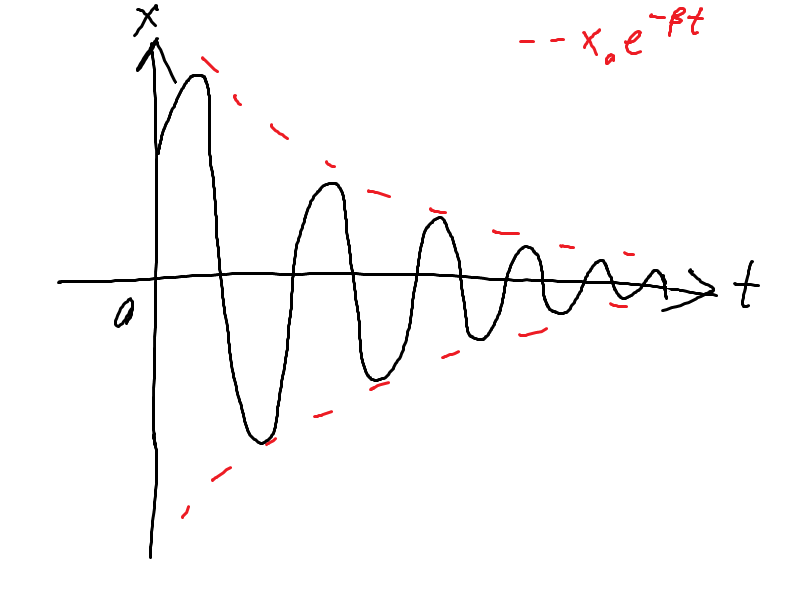
\includegraphics[width=0.33\linewidth]{fig/under-dump.png}
\caption{欠阻尼时的运动}
\label{fig-under-dump}
\end{figure}

$\beta$比较大时,$\Delta<0$,$\omega=\rmi \beta \pm \rmi \sqrt{\beta^2-\omega_0^2}$。根据解的线性叠加可以得到$x=A \rme^{\rmi (\rmi \beta+\rmi \sqrt{\beta^2-\omega_0^2}) t}+B \rme^{\rmi (\rmi \beta-\rmi \sqrt{\beta^2-\omega_0^2}) t}=A \rme^{-(\beta+\sqrt{\beta^2-\omega_0^2})t}+B \rme^{-(\beta-\sqrt{\beta^2-\omega_0^2})t}$。这种情况叫作过阻尼,小球的运动是两个指数衰减的叠加,而$A$和$B$要求都是实数。

$\beta$刚好不大不小时,$\Delta=0$,$\omega=\rmi \beta$,这种情况叫作临界阻尼。奇怪的事情出现了:二阶微分方程的通解必须有两个待定的常量,现在$\omega$只有一个解,怎么办?

我们要把猜解的形式换一下:$x=(A+B t)\rme^{-\beta t}$,代入微分方程,经过一坨求导和合并同类项得到$(A+B t)\rme^{-\beta t} (\omega_0^2-\beta^2)=0$,所以我们猜出来的这个解确实满足原方程,而且只有在临界阻尼的情况下才能这么猜解。到这里为止这个方程就解完了。

如果$\beta=0$,那么欠阻尼和过阻尼的运动都会变成简谐振动,而临界阻尼的运动会变成匀速直线运动。

要注意的是,指数衰减不能严格达到零,实际操作中一般认为小于一个很小的数(比如初始位移的1\%)就算运动停止,而且实际上的阻力也不严格与速度成正比。

【练习】自己把这个方程解一遍,如果能解出来那么之前的东西应该都懂了。
\section{受迫振动}
如果在弹簧振子上再加一个外力$f(t)=m a_0 \sin \omega t$,运动方程就是
\begin{equation*}
x''+2 \beta x'+\omega_0^2 x=a_0 \sin \omega t
\end{equation*}

这是一个非齐次方程,也就是说它的右边是有东西的。非齐次方程的困难之处就在于,没有一种通用的方法来猜解,需要根据方程右边的东西看着办。

通过物理实验我们已经知道,受迫振动的频率与外力相同,那么可以猜$x=A \sin \omega t+B \cos \omega t$,$A,B$都是实常量。代入方程得到
\begin{align*}
-\omega^2 A \sin \omega t-\omega^2 B \cos \omega t+2 \beta \omega (A \cos \omega t-B \sin \omega t)+\omega_0^2 (A \sin \omega t+B \cos \omega t)&=a_0 \sin \omega t \\
((\omega_0^2-\omega ^2)A-2 \beta \omega B)\sin \omega t +(2 \beta \omega A+(\omega ^2+\omega_0^2)B)\cos \omega t&=a_0 \sin \omega t
\end{align*}
\begin{equation*}
\begin{cases}
(\omega_0^2-\omega ^2)A-2 \beta \omega B=a_0 \\
2 \beta \omega A+(\omega ^2+\omega_0^2)B=0
\end{cases}
\end{equation*}

解得$A=\frac{(\omega_0^2-\omega ^2) a_0}{(\omega_0^2-\omega ^2)^2+(2 \beta \omega)^2}$,$B=\frac{2 \beta \omega a_0}{(\omega_0^2-\omega ^2)^2+(2 \beta \omega)^2}$,总振幅为$\sqrt{A^2+B^2}=\frac{a_0}{\sqrt{(\omega_0^2-\omega ^2)^2+(2 \beta \omega)^2}}$。根号里是$\omega$的二次函数,$\omega$略小于$\omega_0$时,振幅最大。相位的变化比较复杂,有(mei)兴(shi)趣(gan)的同学可以画个图。

但是!我们怎么把常量$A$和$B$解出来了?这里的$A$和$B$并不是待定常量,我们解出的只是一个特解,而不是通解。但是我们发现,如果$x_1(t)$是非齐次方程$x''+2 \beta x'+\omega_0^2 x=f(t)$的解,而$x_2(t)$是对应的齐次方程$x''+2 \beta x'+\omega_0^2 x=0$的解,那么$x_1(t)+x_2(t)$是这个非齐次方程的解。

所以把阻尼振动的通解加上去就是受迫振动的通解。阻尼振动的解会指数衰减,所以经过足够长的时间之后就只剩下受迫振动的特解。

【练习】解方程$x''+2 \beta x'+\omega_0^2 x=b_0 \rme^{-\lambda t}$,想一想应该猜什么样的解。

$\phantom{\text{【练习】}}$解方程$x''+2 \beta x'+\omega_0^2 x=a_0 \sin \omega t+b_0 \rme^{-\lambda t}$。真的要从头开始解一遍吗?
\section{小球、磁场与弹簧}
考虑这样一个问题:在平面内,一个小球质量为$m$,带电$q$,在一个匀强磁场$B$里,并且连着一根弹簧,劲度系数为$k$,忽略原长。把小球的坐标设为$(x,y)$,并且设$z=x+\rmi y$,小球的运动方程可以写成
\begin{equation*}
z''+2 \rmi \beta z'+\omega_0^2 z=0
\end{equation*}

其中$2 \beta=\frac{B q}{m}$,$\omega_0^2=\frac{k}{m}$。洛伦兹力的方向垂直于速度方向,所以$\beta$前面乘了一个$\rmi$。复数只要用乘法就可以表示旋转,所以二维问题经常要旋转某个东西就可以考虑用复数。

按照阻尼振动的解法,这个方程的解是$z=A \rme^{\rmi (-\beta+\sqrt{\beta^2+\omega_0^2}) t}+B \rme^{\rmi (-\beta-\sqrt{\beta^2+\omega_0^2}) t}$,其中$A$和$B$是复常量。也就是说,小球的运动是两个半径和角速度不同的圆周运动的叠加。

到现在为止讲的你可以当作全是扯蛋,至少没有哪个学校的自主招生会直接让你算微积分,但是微积分作为一种处理问题的思想是需要掌握的,这样就不需要苦逼的微元法了。
\section{睡前小故事:解方程有多复杂}
二元一次方程组解起来很简单,三元一次方程组就比较困难了,四元以上的方程组如果暴算的话一般是没有希望的,需要观察方程的特点才能解出来。我们可以想办法描述一下解方程的复杂程度。考虑一个$n$元一次方程组:
\begin{align*}
a_{1 1} x_1+a_{1 2} x_2+\dots+a_{1 n} x_n&=c_1 \\
a_{2 1} x_1+a_{2 2} x_2+\dots+a_{2 n} x_n&=c_2 \\
&\dots \\
a_{n 1} x_1+a_{n 2} x_2+\dots+a_{n n} x_n&=c_n
\end{align*}

假设你用一台很慢的电脑来解方程,它每秒可以算一次加法、减法、乘法或者除法。

首先用第一个方程表示出$x_1$:$x_1=\frac{c_1}{a_1}-\frac{a_2}{a_1} x_2-\frac{a_3}{a_1} x_3-\dots-\frac{a_n}{a_1} x_n$。每算一次$\frac{c_1}{a_1}$之类的系数要1秒,总共要$n$秒。

然后把$x_1$代入到第二个方程,这样$x_2$的系数就变成了$-a_{2 1} \frac{a_2}{a_1}+a_{2 2}$,算一次乘法一次加法要2秒,算$n-1$个$x$的系数要$2n-2$秒。

把$x_1$代入到后面的$n-1$个方程里总共要$(2n-2)(n-1)=2n^2-4n+2$秒,加上前面的$n$秒是$2n^2-3n+2$秒。这样$x_1$就从整个方程组里消掉了,剩下$n-1$元一次方程组。

这样的步骤要进行$n$次,总共需要$\sum_{i=1}^n(2i^2-3i+2)=\frac{2}{3} n^3-\frac{1}{2} n^2+\frac{5}{6} n$秒。现在终于解出了一个$x_n$,然后要把它代到上面的式子里解出其他$x$,但是先不管这个。

现在的电脑可以解成千上万个方程联立的方程组。当$n$很大的时候,可以不管一次和二次项,甚至不管三次项的系数$\frac{2}{3}$,所以说$\frac{2}{3} n^3-\frac{1}{2} n^2+\frac{5}{6} n$是一个复杂度为$O(n^3)$的函数。

举几个栗子,$x^3+2x^2+3x$和$4x^3+\frac{5}{x}+6 \sin x$都是$O(x^3)$的函数。当$x$很大的时候,$O(x^3)$的增长速度远大于$O(n^2)$。

$\exp x$的增长速度比任何$x^a$($a$为正数)都大,而$\ln x$的增长速度比任何$x^a$都小。$x^x$的增长速度比$\exp x$还大。

复杂度理论可以帮我们优化做一些事情的方法。比如计算多项式$P(x)=a_0+a_1 x+a_2 x^2+\dots+a_n x^n$,如果一项一项算,第一项是常数,第二项需要一次乘法,第三项需要两次乘法……最后一项需要$n$次乘法,加起来需要$n$次加法,总共需要$\frac{1}{2} n^2+\frac{3}{2} n$秒,复杂度为$O(n^2)$。

但是如果这样算:$P(x)=a_0+x (a_1+x (a^2+\dots))$,那么只需要$2 n$秒,复杂度为$O(n)$。也就是说,把$x^a$记下来,下次要算$x^{a+1}$只要乘一次$x$,而不用从头开始乘。这种方法叫作\emph{秦九韶算法},在国外则叫\emph{霍纳算法}。

一件事情的复杂度是对给定的基本操作而言的,如果你有一台牛逼的电脑可以在一秒钟内算一个多项式,那当我没说。
